
% ===================================================================
% Presentación con Latex Beamer -> EN proceso de modificación -> CCF
% ===================================================================
\documentclass[9pt,xcolor=svgnames]{beamer}
%\documentclass[handout,xcolor=svgnames]{beamer} %Version imprimible
% -------------------------------------------------------------------
\usepackage{paquetes}
% -------------------------------------------------------------------
\usepackage{modo}
% -------------------------------------------------------------------

% Comienza el documento
\begin{document}
% Tikz -> Imágenes
\tikzstyle{every picture}+=[remember picture]
% Entorno matemático
\everymath{\displaystyle}

% Transparencia de Inicio -> Título
\begin{frame}
 \titlepage
\end{frame}

\normalsize

% Transparencia de índice
\begin{frame}
 \frametitle{Índice} 
 \transboxin
 \tableofcontents
\end{frame}
  
  
 \section{Introducción}

 \begin{frame}{¿Qué es \LaTeX?}
   \begin{block}{Wikipedia}
     \noindent \LaTeX{} es un \textbf{lenguaje de marcado} para
     documentos, y un sistema de preparación de documentos, formado
     por un gran conjunto de macros de \TeX{}
   \end{block}

   \pause

   \begin{block}{Más normalito...}
     \noindent \LaTeX{} es un ``lenguaje de programación'' que nos
     permite editar documentos con muchas posibilidades, como fórmulas
     matemáticas, tablas y muchos más.
   \end{block}

   \pause
   
   \begin{block}{\textbf{¡IMPORTANTE!}}
     \noindent Los documentos \LaTeX{} usan extensión \texttt{.tex}, y
     son ficheros de texto plano, que luego se compilan, del tipo
     \textbf{WYSINWYG}.
   \end{block}
   
 \end{frame}

 \section{¿Qué podemos hacer con \LaTeX?}
 
 \begin{frame}[fragile=singleslide]{Fórmulas matemáticas facilmente}
   \begin{block}{Media aritmética}
     \[
     \overline{x} = \frac{\sum_{i = 1}^{n} x_i \cdot{} n_i}{n}
    \]

     \noindent El código simplemente sería
     
     \begin{lstlisting}[style=LaTeX]
 \overline{x} = \frac{\sum_{i = 1}^{n} x_i \cdot{} n_i}{n}      
     \end{lstlisting}
      \end{block}
      
      \begin{block}{Orden $O$}
        \[
        O(f) = \{ t:\mathbb{N} \rightarrow{} \mathbb{R}_0^+ | \exists
        c \in{} \mathbb{R}^+, \exists n_0 \in{} \mathbb{N}, \forall n
        \geq{} n_0\cdot t(n) \leq{} c\cdot f(n) \}
        \]

        \noindent Y en el documento \LaTeX{} se vería:

        \begin{lstlisting}[style=LaTeX]
          
 O(f) = \{ t:\mathbb{N} \rightarrow{} \mathbb{R}_0^+ | \exists
 c \in{} \mathbb{R}^+, \exists n_0 \in{} \mathbb{N}, \forall n
 \geq{} n_0\cdot t(n) \leq{} c\cdot f(n) \}
        
        \end{lstlisting}
     
      \end{block}
      
 \end{frame}

 \begin{frame}{Muy bonito, pero...}
   \begin{block}{¿Esto se usa?}
     \noindent Se utiliza bastante, sobre todo en el entorno
     universitario, en especial en facultades de ciencias.
   \end{block}
   \pause
   \begin{block}{No me lo creo}
     \noindent Si no lo sabes, muchas asignaturas de Ingeniería
     Técnica en Informática (ambas especialidades), utilizan \LaTeX:
     \begin{itemize}
     \item Apuntes de Álgebra, Matemáticas Discretas, Cálculo, Métodos Numéricos...
     \item Relaciones de problemas de ADA1, ADA2, POO, ...
     \item Apuntes de teoría y prácticas de Sistemas Operativos 1 y 2,
       así como las transparencias.
     \item Y muchas más.
     \end{itemize}
   \end{block}
 \end{frame}
 
 \begin{frame}
   \begin{block}{¿No es más facil el OOo Writer?}
     \noindent A primera vista, puede parecer que un procesador de
     textos tipo OOo Writer y alternativas comerciales son más fáciles
     de utilizar que algo como \LaTeX{}, donde no ves que vas
     haciendo. Sin embargo, una vez que te habituas descubres que tiene
     muchas ventajas
   \end{block}
 \end{frame}

 \subsection{Ventajas de usar \LaTeX}

 \begin{frame}
   \begin{block}{Algunas ventajitas}
   \noindent La verdad que la lista puede ser interminable, pero a
   grandes rasgos:
   \begin{itemize}
   \item Más facilidad para utilizar fórmulas matemáticas.
   \item Generación automática de índices, apéndices, bibliografias...
   \item Gestión de referencias dentro del documento.
   \item Al ser texto plano, podemos usar herramientas colaborativas
     tipo \textbf{SVN}.
   \item Existen herramientas para generar código \LaTeX{} automáticamente.
   \item Infinidad de paquetes para múltiples funciones
   \item Y mejor paro ya...
   \end{itemize}
 \end{block}

 \pause

 \begin{block}{Pocas desventajas (haberlas haylas)}
   \noindent No todo van a ser piropos a \LaTeX:
   \begin{itemize}
   \item Muy áspero si no se ha programado nunca.
   \item Cuando no compila el documento, los errores no son nada explicativos.
   \item Algo frustrante al principio.
   \end{itemize}
 \end{block}

\end{frame}

\section{¡No puedo esperar!}

  
  \begin{frame}[fragile=singleslide]
\begin{block}
  \noindent El siguiente código, no es más que la arquitectura básica
  de todo documento \LaTeX{}, aunque luego veremos un par de ejemplos
  más reales.
\end{block}
    
      \begin{block}{Documento base}
        
        \begin{lstlisting}[style=LaTeX]
 % ------ Preambulo -------
\documentclass{article}
          
\usepackage[spanish]{babel}
          
\title{Titulo}
\author{Autor}
\date{\today}

% ----- Cuerpo del documento ----
\begin{document}
\maketitle
% ----- Contenido

\end{document}
        
\end{lstlisting}

\end{block}

\end{frame}

\section{Y ahora...}

\begin{frame}
  \begin{center}
    \Huge ¡A trabajar!
  \end{center}
\end{frame}

\section{Y cuando sea mayor, ¿qué puedo hacer?}

\begin{frame}
  \begin{block}
    \noindent Esto que hemos visto no es más que la punta del
    iceberg. Con \LaTeX, podemos hacer muchísimas más cosas:
  \end{block}

  \pause
  
  \begin{block}
    
    \begin{itemize}
    \item Podemos usar \texttt{GNU Plot} para generar gráficas.
      
    \item Añadir nuestro código \LaTeX{} a código generado
      automáticamente por \texttt{Doxygen}
      
    \item Y más cosas...
      
    \end{itemize}
  \end{block}
\end{frame}

\begin{frame}{Conjuntos}
  \begin{center}
    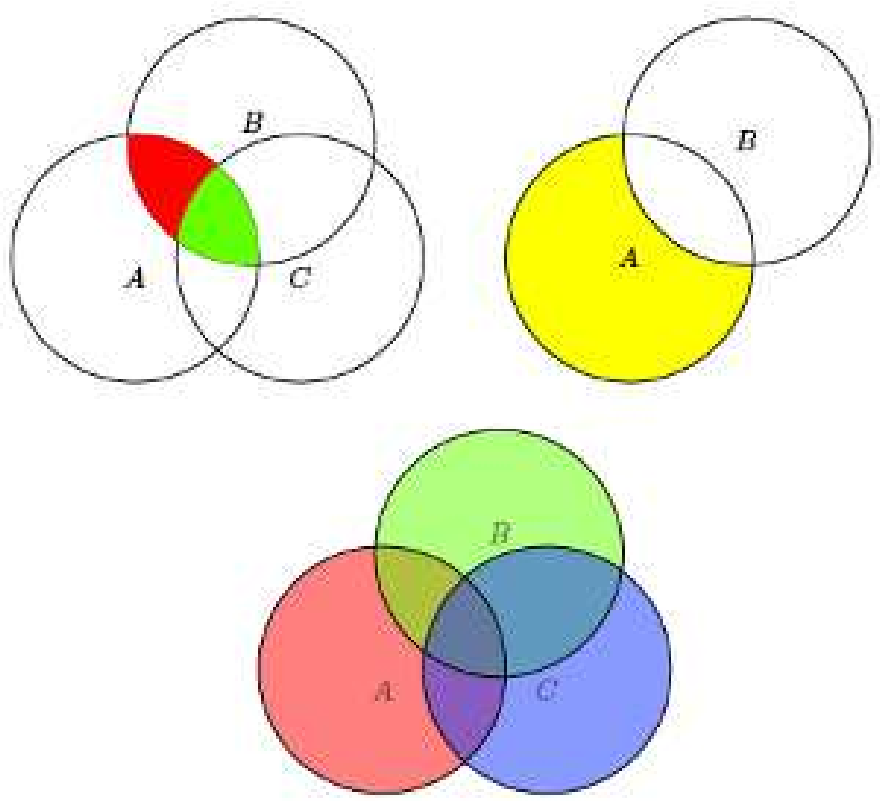
\includegraphics[scale=0.5]{imagenes/sets.pdf}
  \end{center}
\end{frame}

\begin{frame}{Red mental}
  \begin{center}
    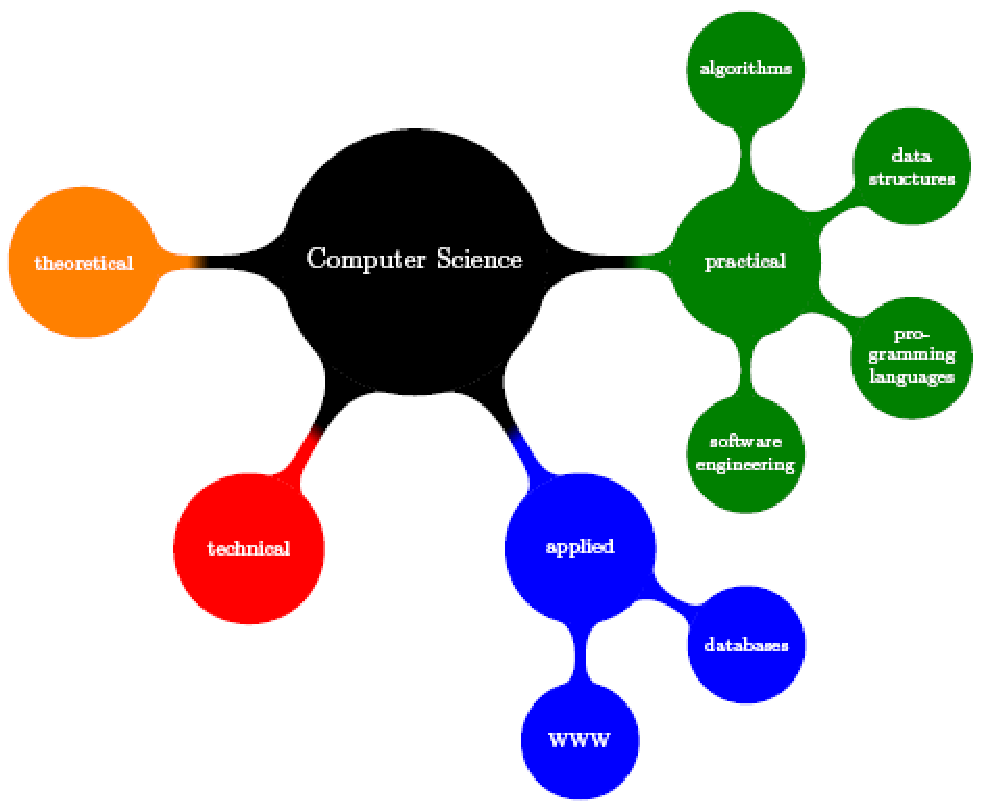
\includegraphics[scale=0.5]{imagenes/red_mental.pdf}
  \end{center}
\end{frame}

\begin{frame}{Partidas de go}
  \begin{center}
    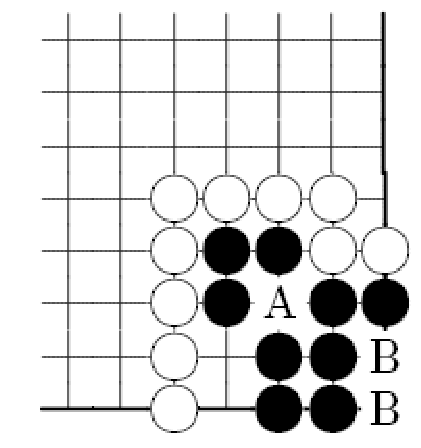
\includegraphics[scale=0.5]{imagenes/go.pdf}
  \end{center}
\end{frame}

\section{Y para terminar...}

\begin{frame}
\begin{center}
\Huge ¡Gracias por asistir!\\
Espero que hayais aprendido y disfrutado.
\end{center}
\end{frame}

\end{document}
  
